\documentclass[a4paper,11pt]{article}
\DeclareUnicodeCharacter{2212}{\ensuremath{-}}
\usepackage{jheppub} % for details on the use of the package, please see the JINST-author-manual
\usepackage{lineno}
\usepackage{bm}
\linenumbers

\arxivnumber{1234.56789} % if you have one

\title{Modeling Falling Backgrounds with Exponential Mixtures}

% Collaborations

%% [A] If main author
%% \collaboration{\includegraphics[height=17mm]{collabroation-logo}\\[6pt]
%%  XXX collaboration}

%% or
%% [B] If "on behalf of"
%% \collaboration[c]{on behalf of XXX collaboration}


% Authors
% The "\note" macro will give a warning: "Ignoring empty anchor...", you can safely ignore it.

%% [A] simple case: 2 authors, same institution
%% \author[1]{A. Uthor\note{Corresponding author.}}
%% \author{and A. Nother Author}
%% \affiliation{Institution,\\Address, Country}

%% or, e.g.
%% [B] more complex case: 4 authors, 3 institutions, 2 footnotes
%% \author[a,b]{F. Irst,\note{Now at another university}}
%% \author[c]{S. Econd,}
%% \author[a,2]{T. Hird\note{Also at Some University.}}
%% \author[c,2]{and Fourth}
%% \affiliation[a]{Institution_1,\\Address, Country}
%% \affiliation[b]{Institution_2,\\Address, Country}
%% \affiliation[c]{Institution_3,\\Address, Country}

\author[1]{Austin Townsend,}
\author[1]{Marc Osherson,}
\author[1]{Mike Hildreth, }
\author[1]{and Stefano Castruccio}
\affiliation[1]{University of Notre Dame,\\
USA}

% E-mail addresses: only for the corresponding author
\emailAdd{atownse2@nd.edu}

\abstract{
Searches for new physics at the LHC often look for a localized excess on a falling background distribution. Several classes of background models have been considered, including polynomials and other parametric families. In this work, we motivate the finite exponential mixture as a flexible class of functions for approximating falling distributions. Using several published results we show that the exponential mixture is competitive for both small ($n=5,036$) and large ($n=28,619,185$) datasets. Finally in simulation studies we demonstrate the exponential mixture's ability to approximate other commonly used functions with small bias and good coverage.
}

\DeclareUnicodeCharacter{2009}{\,}
\begin{document}
\maketitle
\flushbottom


\section{Introduction}
\label{sec:intro}

% Motivation
Searches for new particles are standard in high energy physics. The Large Hadron Collider (LHC) produces environments where new particles may be created by colliding beams of protons that are accelerated to 99.9999991\% the speed of light \cite{LHC_speed}. During a collision, the proton constituents sometimes interact and produce new particles. If a particle is produced and decays within the detector, with visible decay products, one can reconstruct the mass of the parent particle. With enough of these events recorded, we can claim a discovery.

% Backgrounds
The primary challenge in these searches is posed by Standard Model (SM) processes that mimic the signal. These processes are collectively referred to as backgrounds. Because new physics signals are typically rare, they are often obscured by these much more frequent background events. With this setup, searches for new physics employ statistical models containing signal and background components. In the absence of an obvious signal the challenge is to distinguish any possible signal from statistical fluctuations in the background; in this case a proper description of the background model is essential. In this paper, we focus on background models for resonant searches, where signals are represented by local (resonant) deviations on top of a smooth falling background. The signal shapes in non-local (non-resonant) searches vary and require background estimation methods which are out of the scope of this paper.

Background models in resonant searches often rely on data sidebands for identification and range from very flexible to rigid analysis specific background models. Flexible models like polynomials theoretically have low bias, but may need a large number of parameters to achieve this and can be hard to optimize. These models can also be too flexible, fitting the signal if not careful and/or generating nonphysical behaviors in the tails. Previous searches considering polynomials, such as those used to discover the Higgs boson \cite{CMS_Higgs_Discovery, ATLAS_Higgs_Discovery}, avoid these issues by only fitting a portion of the observed mass spectra near the Higgs mass, and masking the signal region when initializing the background parameters. Since the Higgs mass occurs within the bulk of the background, this ensures that the background model is well constrained by the data sidebands. However, other analyses extend their search space to the tails, looking for signals at the far ends of distributions where no sidebands are available. These analyses require better extrapolation techniques.

Analysis specific background models are often more rigid, avoiding some of the drawbacks that come with very flexible models like polynomials. The underlying theory describing the particle interactions is complicated enough that there are generally no closed form expressions for describing these backgrounds, but still there are some good approximations. The most famous example is the dijet function. It has been used since the 1990's by the CDF and D\O\ collaborations and more recently by CMS and ATLAS \cite{Harris:2011bh} to describe the invariant masses of particle jets in hadron colliders, searching for new resonances or other anomalous behavior. This function is motivated by leading order quantum chromodynamics (QCD) and the mass dependence of parton distribution functions \cite{Harris:2011bh} but also includes ad-hoc terms which are used to improve the fit to the data. This function works on existing datasets, but since it relies on a number of approximations, it is likely to need updating as datasets grow in size.

Other searches will use objects such as photons or electrons. Backgrounds in these kinds of searches tend to be more complicated, as the objects can be real SM photons/electrons or they can be signatures faked by other objects like hadronic jets. Despite this, the dijet function (or a version with a smaller number of parameters) is often considered. To combat the bias associated with the assumption of a particular functional form, more recent analyses \cite{CMS_high_mass_diphoton} will often consider a number of background functions simultaneously using the discrete profiling method \cite{discrete-profiling}. These functions are typically chosen from a larger set of function classes, which can be extended with more parameters. In these cases, researchers are typically interested in finding function classes that approximate the spectra with the smallest number of parameters, using test-based model selection methods.

In this paper, we consider the finite exponential mixture as an alternative approach to modeling smoothly falling backgrounds. We treat the exponential mixture as an approximation, including additional parameters as determined by the data. We show the fits for several published datasets and compare the performance against traditional models. This exponential mixture assumes that the true background density is completely monotonic, which is not always the case. However, we find that the exponential mixture can match the performance of previous methods in datasets that vary widely in dataset size (from $n=5,036$ to $n=28,619,185$). On pseudo-datasets simulated from historically-used functions we show that, with an appropriate model selection metric, the exponential mixture has small bias and exceptional coverage in the bulk, making the use of additional functions unnecessary. The exponential mixture is flexible enough to generalize to different datasets, while rigid enough to avoid most overfitting.

In the next section, we introduce the finite exponential mixture and our parameterization with the model selection procedure and its justification. We also discuss some issues related to implementation and global optimization. In sections \ref{sec:example1} and \ref{sec:example2} we fit the exponential mixture to two published datasets, comparing with the original methods. In section \ref{sec:toys} we generate pseudo-datasets using the set of functions considered in \ref{sec:example2} and compare the bias, coverage, and spurious signal of those models with the exponential mixture. Finally in section \ref{sec:discussion} we summarize the results and discuss several considerations, extensions, and areas for future research.

\section{Exponential Mixtures}
\label{sec:emm}

The density of a general single parameter mixture ($\theta$) is given by
\begin{equation}
\label{general_mixture}
f(x) = \int p(\theta) p(x | \theta) d\theta \, ,
\end{equation}
where $p(x|\theta)$ is the base density (exponential in our case), and $p(\theta)$ is the mixing density. In general $p(\theta)$ can be any density function defined in the domain of $\theta$, although it is commonly estimated non-parametrically as a discrete distribution with $k$ supports. This discrete estimate of $p(\theta)$ can be written as:
\begin{equation}
\label{sum_approx}
p_k(\vec\theta)=\sum_{i=1}^k w_i \delta(\theta-\theta_i),
\end{equation}
where $\vec\theta$ is the vector of the $k$ supports $\theta_i$, $\delta(\cdot)$ is the Dirac delta distribution and $\sum w_i=1$ for normalization. Substituting \ref{sum_approx} into \ref{general_mixture} we find the common form of the finite mixture density:
\begin{equation}
\label{finite_mixture}
f_k(x|\vec\theta) = \sum_{i=1}^k w_i p(x | \theta_i) \, .
\end{equation}

Instead of monotonicity, if we make the stronger assumption of complete monotonicity\footnote{A function is completely monotonic if
\begin{equation}
(-1)^n f^{(n)}(x)\geq 0
\end{equation}
for all $n \in \{0,1,2,\ldots\}$. This means that the function is non-negative, non-increasing, convex, and so on.}, then by Bernstein's theorem on monotone functions \cite{bernstein}, the true density is an exponential mixture.  

The class of completely monotonic functions is closed under addition and multiplication \cite{completetly_monotone}. This class of functions includes $f(x)=a$, $f(x)=1/(a+x)^b$, $f(x)=e^{-xt}$, $f(x)=(1+x)^{1/x}$, and $f(x)=\log(1+x)/x$, to name a few. For functions in this class, the exponential sum is guaranteed to converge uniformly \cite{McGlinn_1978}. This class does not include functions like the falling tail of a Normal distribution, for example, though the approximation becomes better if one restricts the domain to be sufficiently far from the mean.

Using eq. \ref{finite_mixture} we can write the exponential mixture density as:
\begin{equation}
f_k(x) = \sum_{i=1}^k w_i e^{-\beta_i x} \, ,
\end{equation}
where $\beta_i$ is identified as the rate parameter of the exponential distribution which is now restricted to $[0,\infty)$. To enforce the condition that the weights $\vec{w}$ sum to 1, the parameters are constructed from a set of free parameters $\vec{v}$ with $k-1$ degrees of freedom using the softmax function:
\begin{equation}
\label{softmax}
w_i = \frac{e^{v_i}}{\sum_{j=1}^{k}e^{v_j}} \, ,
\end{equation}
where $v_1=0$ and $v_{i\neq 1} \in (-\infty,\infty)$.

% ROOT MLE
The model parameters are estimated from data distributions using maximum likelihood estimation (MLE) using Python distributions of the \texttt{RooFit}~\cite{RooFit} library within the \texttt{ROOT} framework \cite{ROOT}. The use of the \texttt{ROOT} framework is motivated by its widespread use in particle physics research. The optimization uses the \texttt{MINUIT} package \cite{Minuit2} with the \texttt{MIGRAD} optimization algorithm. \texttt{MIGRAD} is a variable-metric method with inexact line search, a stable metric updating scheme, and checks for positive-definiteness.

% RooFit range dependence
\texttt{RooFit} will calculate a normalization for the density which depends on the range $(X_{\min},X_{\max})$ of the observable $X$ which makes sense for observables that have physical constraints. We found that the model selection answer depends on $X_{\max}$ even in the case where $X_{\max}>\max(X)$. In particular, we found that $X_{\max}$ near, but greater than $\max(X)$ prefer more complex models with densities that fall off very slowly. We set the \texttt{RooFit} range based on the range of possible observations that we would like to use to constrain our model which includes regions ($X>\max(X)$) of zero events up to a threshold determined by the beam energy, the physics of the underlying interactions, and the model used. Generally this decision will require some consideration if the data are near the physical threshold; however, for simplicity we choose an upper threshold of 10 TeV below the beam's 13 TeV center of mass energy.

% Convexity and Identifiability
Mixture models are notoriously non-convex. One trivial source of non-convexity comes from the fact that each exponential term is equivalent. This is known as label switching and means that every minimum [In the MLE?] is replicated $k!$ times. In addition, false minima can be found when one part of the rate space has too many supports while other parts of the space have too few. This can be seen in the case of the 2 component mixture; if the supports are initialized close together they will become trapped in a false minimum, effectively producing the $k=1$ model. This problem becomes more of an issue as the number of components increases. Given the low dimensionality required for the datasets considered in this paper ($k<6$) we use random restarts to approximate the global minimum, using more restarts for larger $k$. For more advanced methods, see \cite{split-and-merge}.

% Model Selection
The number of components needed to fit a dataset is determined from that dataset. In contrast to Gaussian mixtures or polynomials, exponentials are rigid, minimizing the risk of overfitting statistical fluctuations in the background or localized signals. An exception is that this model [Describe why this is.  It's obviously not part of the exponential mixture but something introduced to describe physics and thresholds.] is free to add a component near the lower threshold which falls off very fast. To fix this, we impose an upper threshold on the rate parameters which is set to be 50 times the rate of a single exponential estimated by $1/(\mathbb{E}(X)-X_{\min})$. We use this reference rate to define a normalized set of rate parameters for the exponential rates so that the initialization can be robust to different datasets. With this transformation, the rate parameters tend to be between 0.5 and 2.5.

Model selection methods vary depending on the goal of the analysis. If the components of the model have physical significance it may be more useful to use conservative test based methods like the likelihood ratio test (LRT). In our case, we are not interpreting the parameters of the exponential mixture. Instead, we are using this model only as a means of flexibly approximating some unknown density. Following the discussion of McLachlan and Peel (chapter 6.1.1) \cite{finite-mixture-models}, we restrict our set of model selection metrics to the penalized likelihood measures AIC [Define] and BIC [Define]. In Section \ref{sec:toys} we compare the bias and coverage using these metrics and find AIC to be the least biased with the best coverage. Therefore, we will use AIC to determine the number of exponential components.

As we approach or surpass the number of components needed to model a dataset, we find that the likelihood becomes very flat as a result of the optimization of exponential components with very small weights. In some cases the minimizer will stop and report $\text{status}=3$, which means that the estimated distance to the minimum is above the pre-defined threshold. In these cases, it can be useful to simply run the optimization again with the parameters starting at the values returned by the last optimization attempt. Depending on the dataset and initialization, this may take 50 to 100 attempts until the minimizer converges to an acceptable minimum. It is possible that this is a sign that we have added too many components or that some of the other components are too close together (from bad initialization). Regardless, we allow for a number of retries for every random restart to improve the rate of fits that find an acceptable minimum.

\section{ATLAS Dijet Spectrum} \label{sec:example1}

% Introduce dataset
The dataset utilized in this section was collected by the ATLAS experiment at the LHC during the Run 2 data-taking period, spanning from 2015 to 2018 \cite{ATLAS_Dijet}. The publication uses several signal regions defined by the half rapidity separation between the two leading jets $y^*= (y_1 − y_2)/2$, where $y_1$ and $y_2$ are the rapidities of the leading and subleading jets. For this example, we use the dataset defined by $|y^*|<0.6$.

% Dijet function
This analysis used a sliding window fit with the dijet function. The dijet function is given by:
\begin{equation}
f_D(x) = p_0(1-x)^{p_1}/x^{p_2+p_3\log x},
\end{equation}
where $x=m_{jj}/\sqrt{s}$ for the two jet invariant mass $m_{jj}$ and the center-of-mass energy $\sqrt{s}=13$ TeV. We do not replicate the sliding window fit method here, instead fitting the entire spectrum at once for our comparisons.

% Binning explanation
The dataset available on \texttt{HEPData} \cite{Maguire_2017} is binned. Datasets in high energy physics can be very large, causing fits to the original (unbinned) dataset to be time consuming. In these cases, it is common to bin the data fine enough to not lose information, but wide enough that fits converge in reasonable times. The bin widths in this case are determined by the dijet invariant mass resolution, which broadens at higher values. The binned likelihood is then given by the product of Poisson probabilities:
\begin{equation}
    L(\beta) = \prod_b \text{Pois}(n_b|n_{f,b}),
\end{equation}
where $b$ is the bin, $n_b$ is the number of observations in bin $b$ and $n_{f,b}$ is the expected number of events in bin $b$. The expected number of events is given by:
\begin{equation}
    n_{f,b} = \int_{b_-}^{b_+} f(m|\beta)dm,
\end{equation}
where $b_-$ and $b_+$ are the lower and upper edges of bin $b$.

% Implementation
    % Zero overflow bin
    % Number of random restarts.
    % Model selection

The binning provided on $\texttt{HEPData}$ only includes a single, small width bin following the last bin with non-zero entries. Because of the model selection's dependence on the upper threshold of the fit, we add an additional bin with zero entries that extends to 10 TeV as discussed in the previous section. Since this dataset is large, we will likely need higher $k$ to adequately model it. Higher $k$ implies more false minima, so we use 80 random restarts per model with 100 retries each fit. This is a conservative choice; it is possible that fewer restarts will result in the same solution. In Figure \ref{fig:dijet_AIC_BIC} we show the AIC (and BIC) scores for various $k$. The model with the best AIC has four components.

\begin{figure}
    \centering
    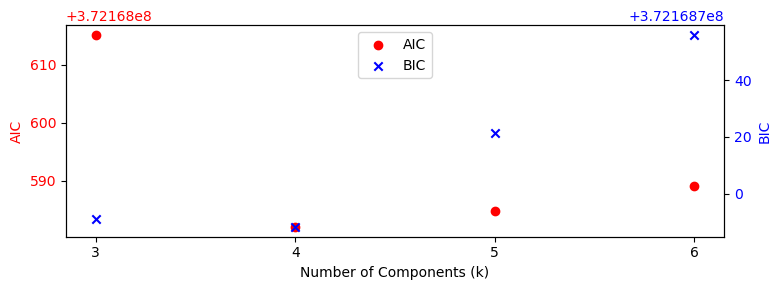
\includegraphics[width=\linewidth]{dijet_AIC_BIC.png}
    \caption{AIC (red dot) and BIC (blue x) scores for exponential mixtures on the ATLAS dijet dataset for $k=3,4,5,6$ mixture components.}
    \label{fig:dijet_AIC_BIC}
\end{figure}

\begin{figure}[h]
    \centering
    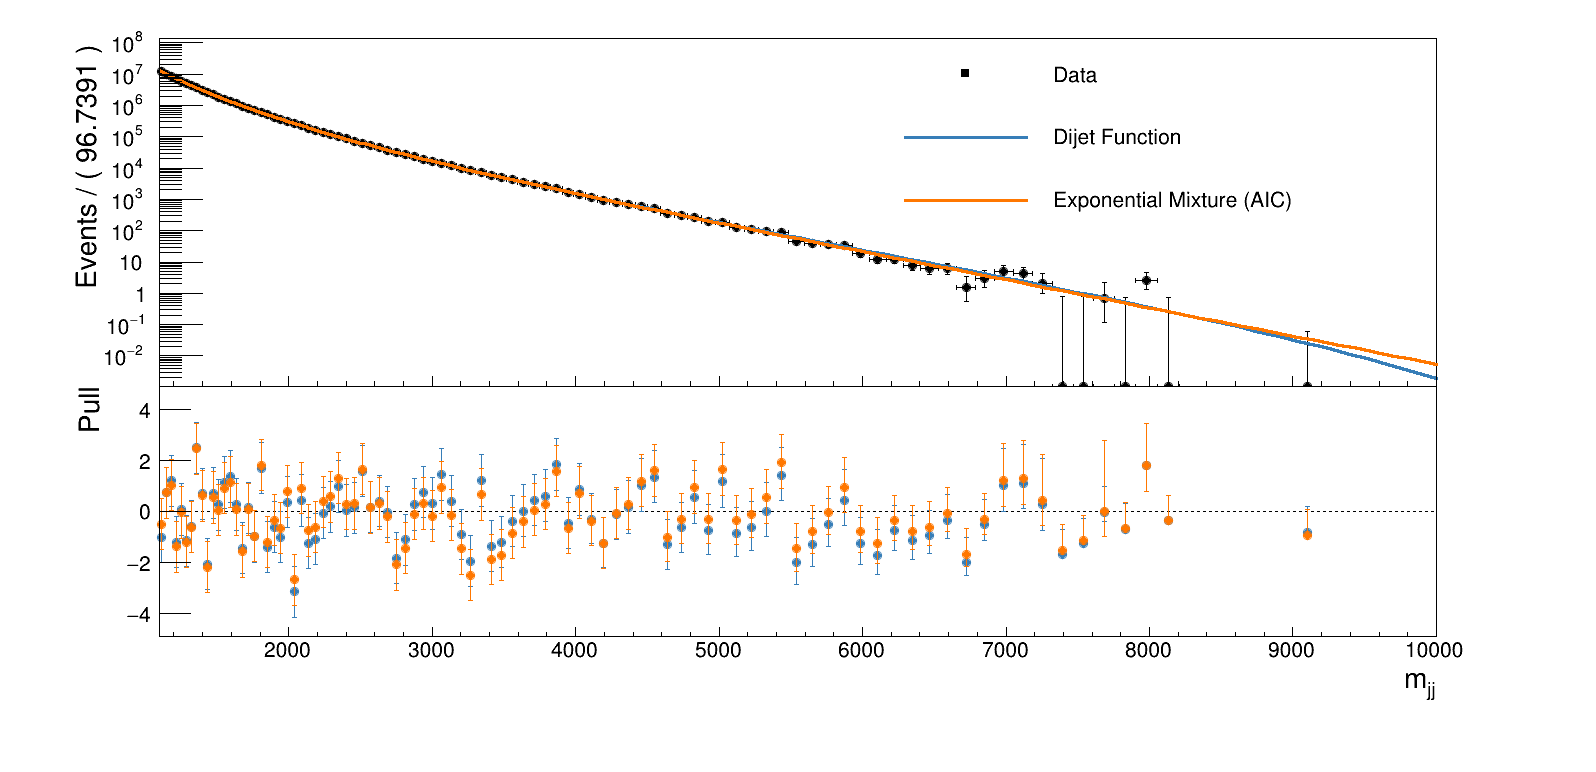
\includegraphics[width=\linewidth]{dijet_fit.png}
    \caption{Fit of Dijet function and exponential mixture to ATLAS Run 2 Dijet dataset. The pulls (normalized residuals) are calculated as $(n_b-n_{f,b})/\sqrt{n_b}$ where $n_b$ is the number of events in bin $b$, $n_{f,b}$ is the expected number of events using function $f$.}
    \label{fig:dijet_fit}
\end{figure}

\begin{table}[h]
\centering
\begin{tabular}{lcc}
\hline
Model & AIC & BIC \\
\hline
Dijet Function & 372168582.25 & 372168627.76 \\
Exponential Mixture (AIC) & 372168581.97 & 372168688.16 \\
\hline
\end{tabular}
\label{tab:dijet_AIC_BIC}
\caption{[This table has no caption. Also, the numerical values are less than elucidating.]} 
\end{table}

The fit of the dijet function and the 4 component exponential mixture to the Dijet dataset is shown in figure \ref{fig:dijet_fit}. Looking at the pull plot we see that the two functions provide similar estimates throughout the mass range. The AIC and BIC scores are shown in Table \ref{tab:dijet_AIC_BIC}. [Weird numbering - why isn't this Table 1?] The exponential mixture provides a better fit in terms of AIC and the dijet function provides a better fit in terms of BIC. 

% The tradeoff is then between a small parameter model which is theoretically motivated and a large parameter flexible model which may have reduced sensitivity if the Dijet function provides a better description. However, we show later in Figure \ref{fig:spurious} that the variance in the exponential mixture's predictions are not much larger than that of the true data generating model.

\section{CMS High Mass Diphoton Spectrum} \label{sec:example2}

% Indroduce dataset
In this section, we consider the run 2 dataset published by CMS in the high mass diphoton final state \cite{CMS_high_mass_diphoton}. The CMS detector is a general-purpose apparatus built in and around a large-bore superconducting solenoid, which generates a 3.8 T magnetic field containing the inner tracking system and the calorimeters. For diphoton resonance searches, the most critical subsystem is the electromagnetic calorimeter (ECAL), composed of more than 75,000 lead tungstate (PbWO$_4$) crystals. This homogeneous calorimeter provides coverage in the barrel ($|\eta|<1.479$) and endcap ($1.479<|\eta|<3.0$) regions, delivering the exceptional energy resolution and fine granularity necessary to give precise estimates of the invariant mass. For simplicity we will only use the sample ($n=5,036$) where both photons are in the ECAL barrel region.

The background estimate for this analysis uses the discrete profiling method with the following functions:
\begin{align} \label{eq:dipoton_fns}
    f_1(x)&=p_0x^{p_1+p_2\log(x)}, \\
    f_2(x)&=p_0e^{p_1x}x^{p_2}, \\
    f_3(x)&=p_0(1+xp_1)^{p_2}, \\
    f_4(x)&=p_0(1+xp_1)^{p_2+p_3x},
\end{align}
where $x=m_{\gamma\gamma}/\sqrt{s}$, $m_{\gamma\gamma}$ is the invariant mass of two photon system and $\sqrt{s}$ is the center-of-mass energy. 

With the published parameter estimates on \texttt{HEPData} we can see that $f_2$ and $f_3$ are completely monotone functions. The first function $f_1$ has completely monotone components but the term $x^{p_2 \log(x)}$ is not; most departures from complete monotonicity are found at low $x$. The derivatives of function four $f_4$ are more complicated than the other functions but a visual inspection of the derivatives shows no departure from complete monotonicity up to the fourth derivative.

% Implementation
    % Upper threshold
    % Number of random restarts
    % Model selection
While the official HEPData entry for this study provides a binned dataset, the CMS collaboration provided the unbinned data upon request. In this case, the likelihood is given by:
\begin{equation}
    \mathcal{L}(\vec\theta) = \prod_{n=1}^N p(x_i|\vec\theta),
\end{equation}
where $\vec\theta$ are the parameters of the model and $p$ is the probability density function. This sample has a relatively small number of entries, so we use 20 random restarts with 5 retries each. From AIC we determine that the exponential mixture with $k=2$ provides the best fit.

% Show fit, compared with other functions
\begin{figure}[h]
    \centering
    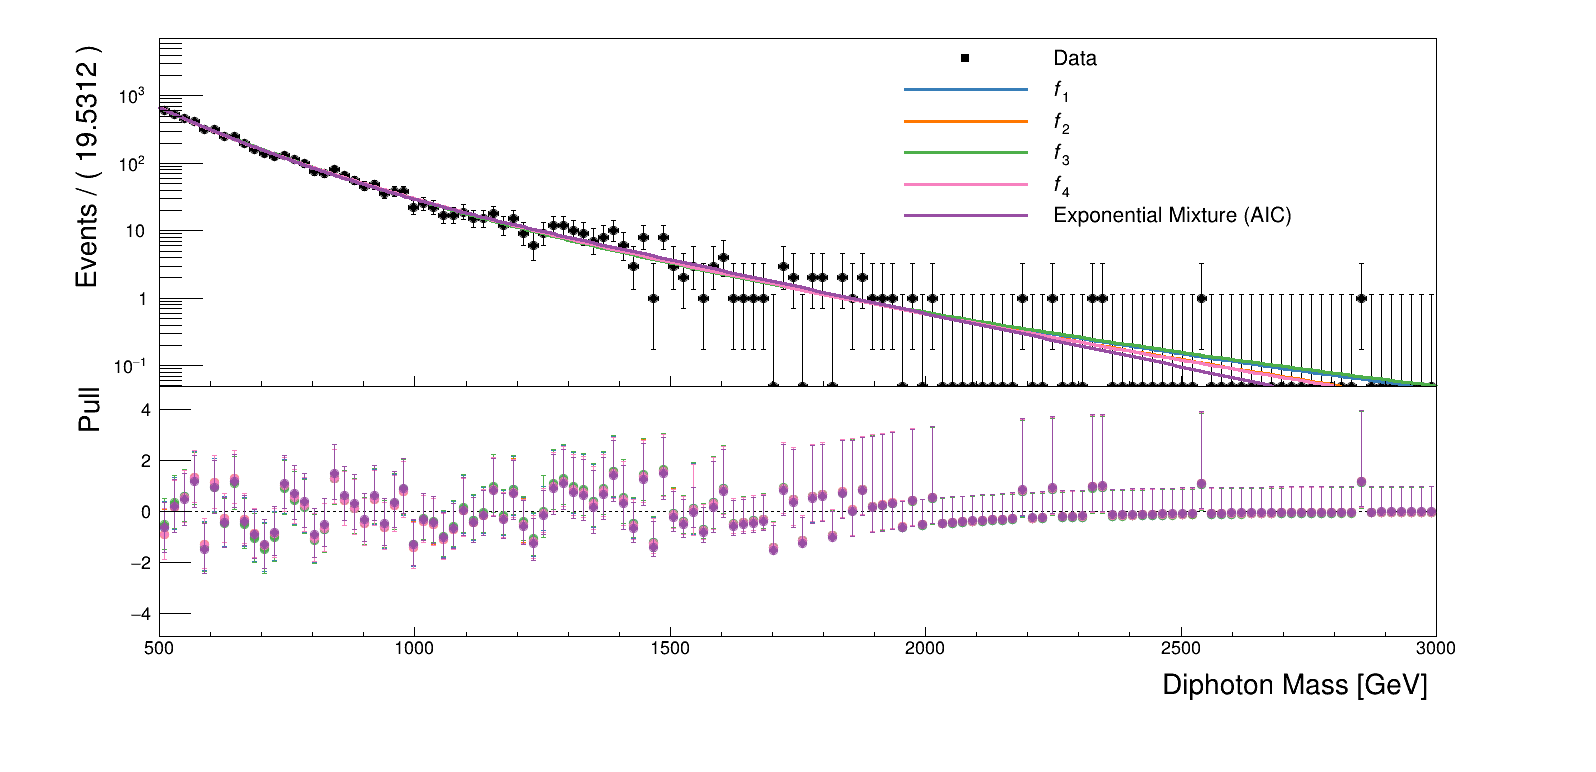
\includegraphics[width=\linewidth]{diphoton_fit.png}
    \caption{Fit of original functions and exponential mixture (AIC) to CMS high mass diphoton dataset. For visualization the data/density functions are binned. The pulls (normalized residuals) are calculated as $(n_b-n_{f,b})/\sqrt{n_b}$ where $n_b$ is the number of events in bin $b$, $n_{f,b}$ is the expected number of events.}
    \label{fig:diphoton_fit}
\end{figure}

\begin{table}[h]
\centering
\begin{tabular}{lcc}
\hline
Model & AIC & BIC \\
\hline
$f_1$ & 62070.4 & 62083.5 \\
$f_2$ & 62068.6 & 62081.6 \\
$f_3$ & 62071.5 & 62084.6 \\
$f_4$ & 62070.4 & 62090.0 \\
Exponential Mixture (AIC) & 62069.7 & 62095.8 \\
\hline
\end{tabular}
\label{tab:diphoton_AIC_BIC}
\caption{[tables need captions]}
\end{table}

% Talk about the figure
Though the fit is performed without binning we bin the dataset for visualization. The fits of all four original functions and the exponential mixture are shown in Figure \ref{fig:diphoton_fit}. From the pull plot we see that the estimates are very similar and that the differences are small relative to the uncertainty of the data in the bins. The AIC and BIC scores are shown in Table \ref{tab:diphoton_AIC_BIC} [again, should be table 2.] where $f_2$ has the smallest AIC followed by the exponential mixture model.

\section{Simulation Studies}\label{sec:toys}

% Introduce toy models
In this section, we will quantify how well the exponential mixtures can approximate the functions in \ref{eq:dipoton_fns}. Results are obtained from fits to a number of pseudo-datasets generated from each function. In each case, the true parameters are obtained via MLE on the CMS high mass diphoton dataset. The number of exponential components used is determined independently for each pseudo dataset and we show the results using both AIC and BIC. Ultimately, we quantify the agreement in terms of bias, coverage, and spurious signal yield.

% Bias and Coverage
The bias is measured by the average density difference scaled by the standard deviation of the density estimated using the true model. This quantity, the relative deviation ($D(x)$) is given by:
\begin{equation}
    D(x) = \frac{1}{T}\sum_{t=1}^T \frac{f_t(x)-f(x|\hat{\bm{\beta}}_t)}{f_t(x)}
\end{equation}
where $f_t$ is the true density function that is used to generate the pseudo dataset, $f$ is the model that is being tested, and $f(x|\hat{\bm{\beta}}_t)$ is the maximum likelihood estimate of $f$ for the toys dataset $t$.

Figure \ref{fig:bias} shows the relative deviation of the exponential mixture with respect to the four generating functions \ref{eq:dipoton_fns}. Each plot uses a different generating function; the fits to the other three functions are shown for scale. We analyze these plots by focusing on their minima, maxima, and crossing points. A good approximation will cross the true value many times and have less extreme biases. The exponential mixture chosen by AIC has the largest number of crossing points and a bias which is mostly contained within the 1 standard deviation interval of the true model, outperforming the one chosen by BIC. This exponential mixture (AIC) also has among the smallest biases across competing models, but also the most parameters.

\begin{figure}[h!]
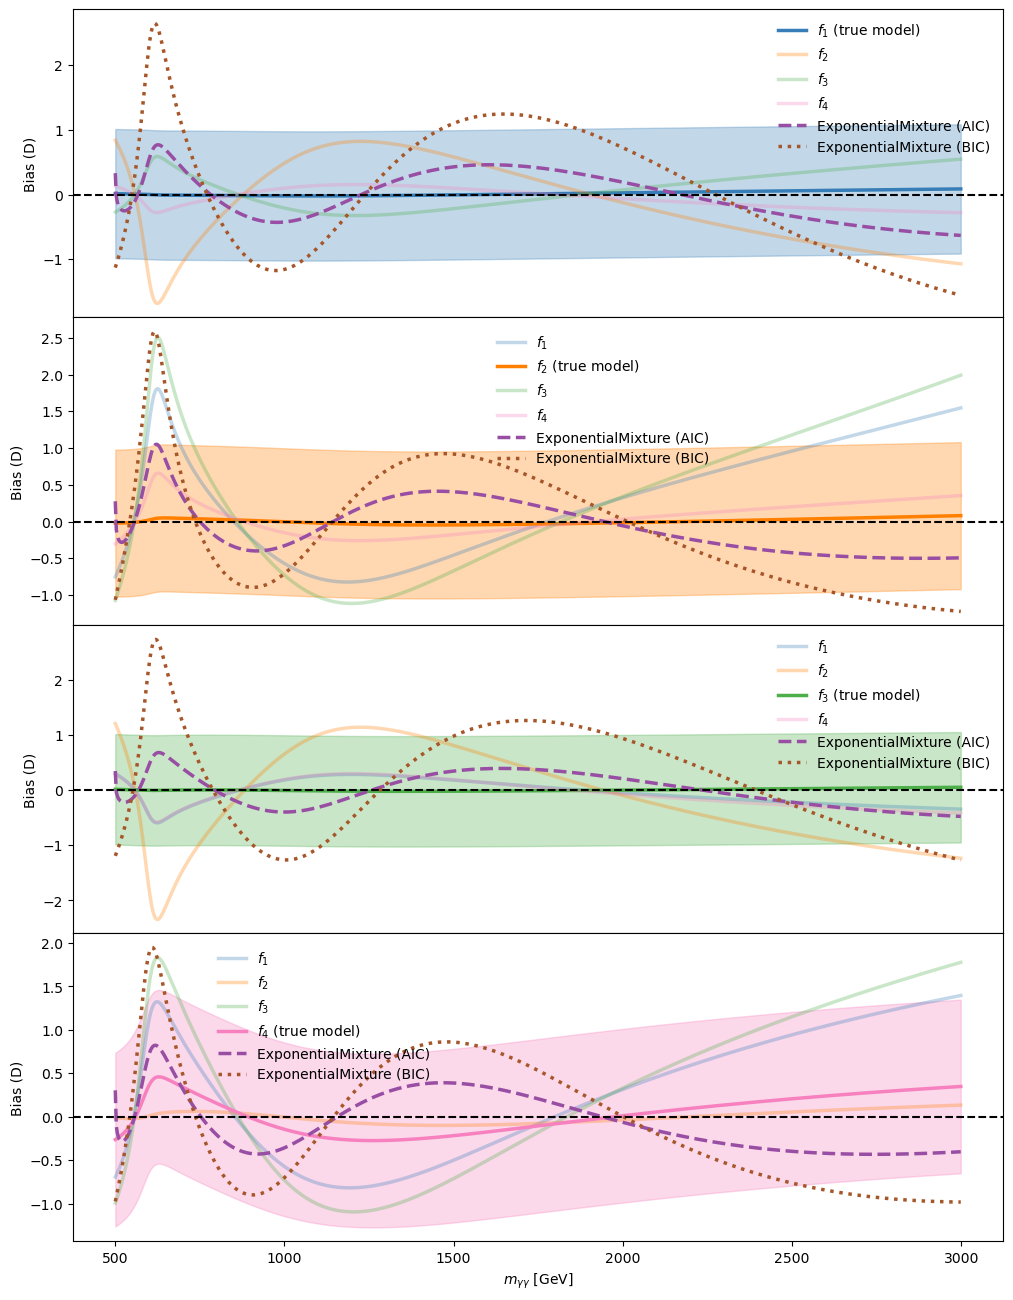
\includegraphics[width=\textwidth]{bias.png}
\caption{Percent deviation of estimated density for various functions. Each row represents approximately 5000 datasets simulated from the true model with $n=5,036$ entries in each. The shaded regions represent the plus/minus one standard deviation band for the true model estimates.}
\label{fig:bias}
\end{figure}

Coverage is a measure of how well the uncertainty in the estimated density covers the true density. Since we are testing exponential mixtures of varying complexity, these fits will often have parameters which are only weakly identified by the data. In these cases the likelihood surface becomes irregular due to label switching and weakly identified parameters, causing Hessian or profile based approximations of the density uncertainty to be unstable. To avoid these issues when estimating the uncertainty in the predicted density, we use the non-parametric bootstrap to estimate our confidence intervals.

To approximate the sampling distribution of the MLE $\hat{f}(x|D)$, we generate a collection of $B$ bootstrap resamples, $\{D_1,D_2,\ldots,D_B\}$, by sampling with replacement from the original dataset D. For each resample, we re-estimate the density to produce a set of bootstrap replicas, $\{\hat{f}(x|D_b)\}_{b=1}^B$. From this set, we construct the empirical $(1-\alpha)$ confidence interval for the density function with linear interpolation.

The coverage of function $f$ for known density $f_t$ and dataset size $n=5,036$ is then estimated by simulating a number of datasets and counting how often the true density is contained within the bootstrap confidence interval. The coverage is thus defined to be:
\begin{equation}
    C(x|f,f_t,T,B) = \frac{1}{T}\sum_{i=1}^T I(x|D_i)
\end{equation}
where $T$ is the number of simulated datasets, $B$ is the number of resamples, and $I$ is the indicator function. The indicator function is defined as
\begin{equation}
    I(x|D) =
    \begin{cases}
        1, & \text{if } f_{t}(x) \in \mathrm{CI}_B(x|f,D), \\
        0, & \text{otherwise},
    \end{cases}
\end{equation}
where $CI_B(x)$ is the bootstrap confidence interval with $B$ resamples.

The coverages are shown in figure \ref{fig:coverage}. As in the bias study, the model selection metrics AIC and BIC are compared, with AIC outperforming BIC again. The exponential mixture chosen by AIC is relatively consistent across all models, maintaining the nominal coverage at least for $m_{\gamma\gamma}<2000$ GeV. In the tails, while the exponential mixture under-covers, it still maintains one of the best coverages among all functions. 

\begin{figure}[h!]
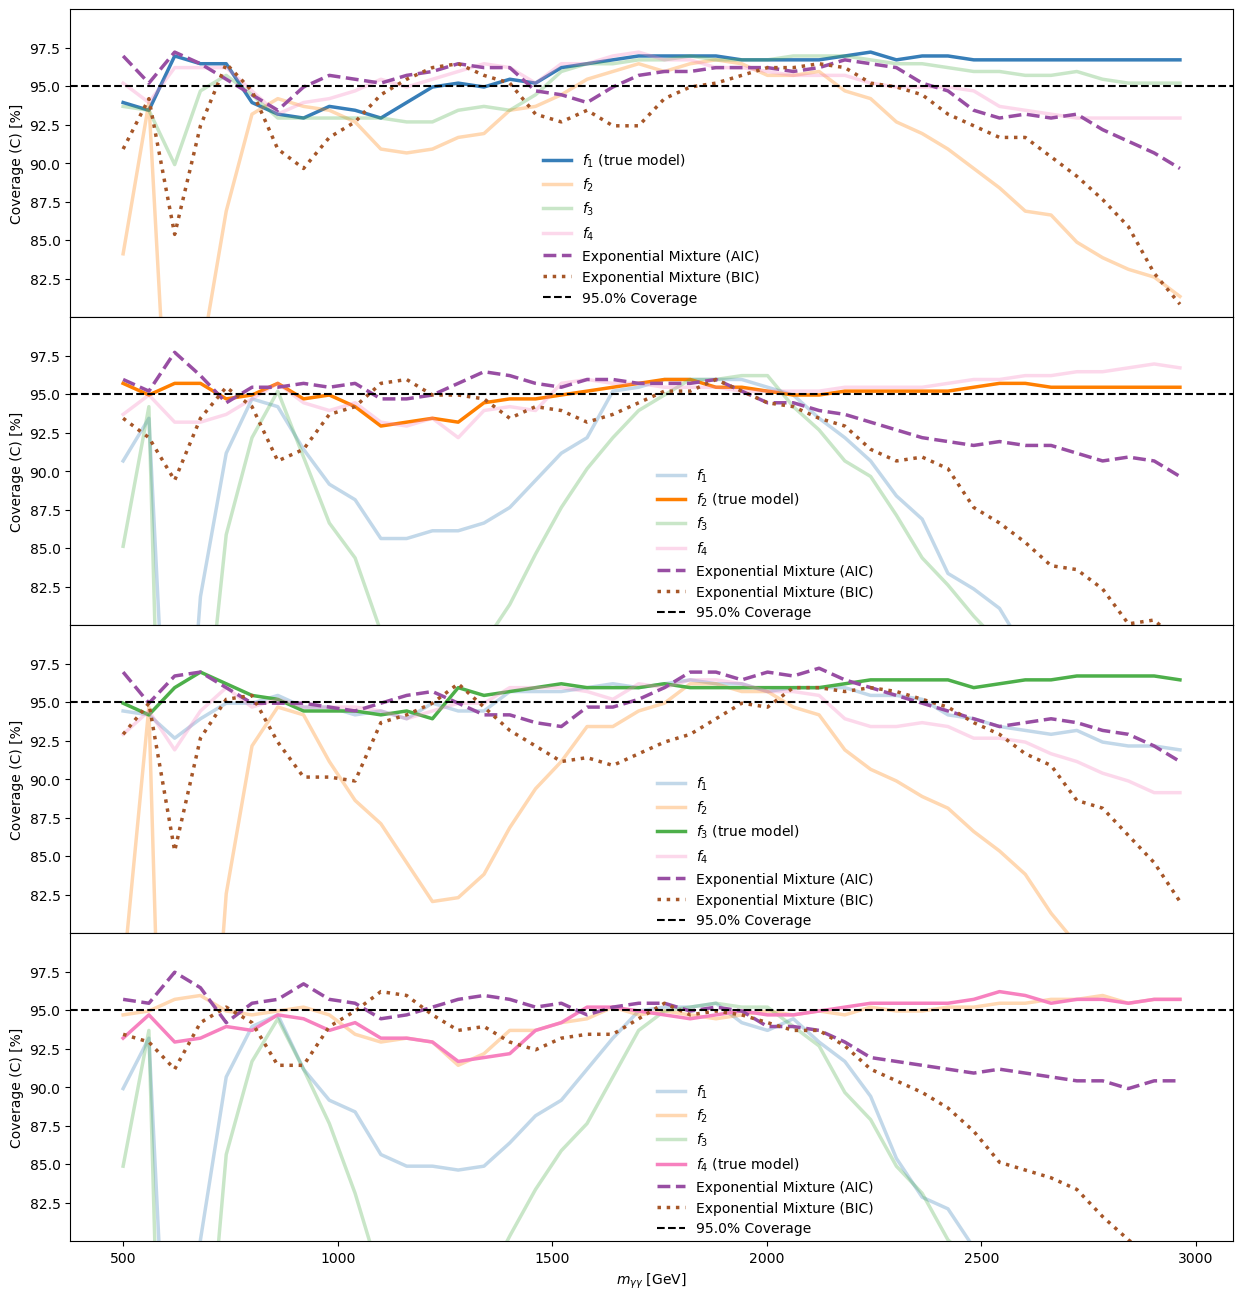
\includegraphics[width=\textwidth]{coverage.png}
\caption{Coverage of estimated density for various functions. Each row represents 400 datasets simulated from the true model with $n=5,036$ entries in each. The 95\% confidence interval is calculated using $B=1000$ bootstraps.}
\label{fig:coverage}
\end{figure}

\begin{figure}
    \centering
    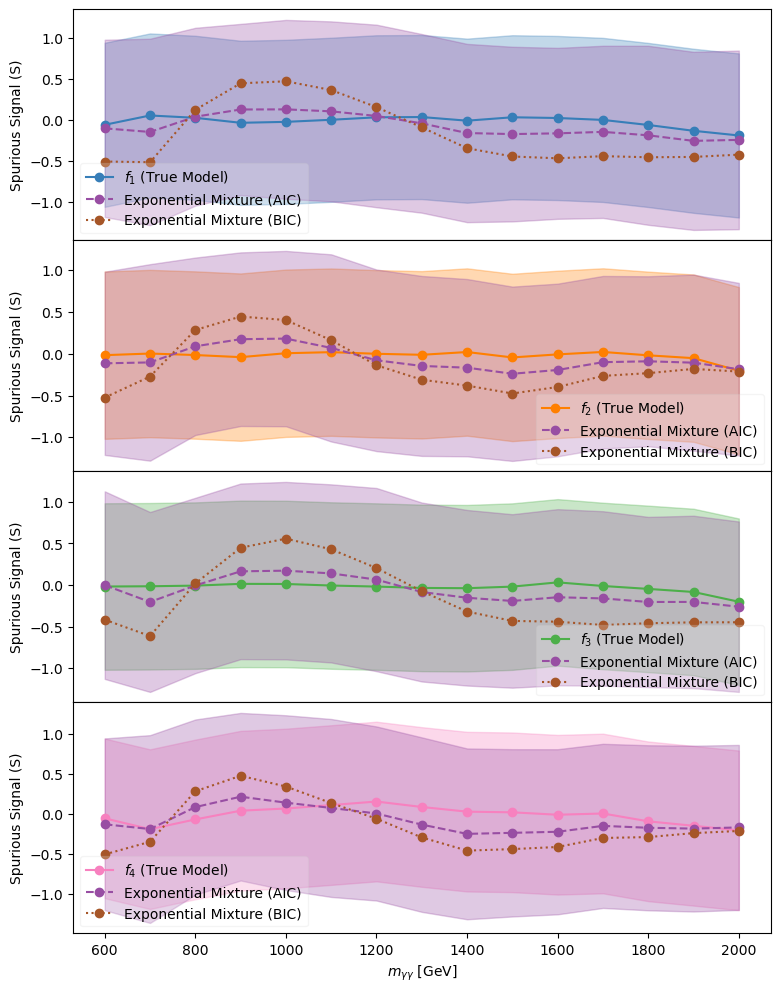
\includegraphics[width=0.9\linewidth]{spurious_signal.png}
    \caption{Shown is the comparison of the (truth normalized) expected signal yield $S(x)$ for several data generating functions and the exponential mixtures. Each point represents the average over 1000 pseudo-datasets, and the bands represent the 1 standard deviation interval. The bands are only shown for the true model and the exponential mixture chosen by AIC. Each subplot represents a different data generating model.}
    \label{fig:spurious}
\end{figure}

Next we compare the spurious signal yield of the data generating models to the exponential mixtures. We fit the pseudo-datasets with a signal plus background model defined by:
\begin{equation}
    f(x)=N_bb(x)+N_ss(x),
\end{equation}
where $N_s$ is the signal yield, $s(x)$ is the signal model, $N_b$ is the number of background events, and $b(x)$ is the background model. In all cases the signal model is defined to be a Normal distribution with variance ranging from 30 to 60 GeV at low and high mass, respectively. We extract the signal yield over 1000 pseudo-datasets for signal mass means from 600 to 2000 GeV.

For each of the 4 data generating functions given above (\ref{eq:dipoton_fns}), we compare the signal yields given by the exponential mixtures (AIC and BIC) to the signal yields given by the true models. Because the signal yields in the tail are much smaller than those in the bulk we use the normalized signal yield given by:
\begin{equation}
    S(x) = \frac{1}{T\sigma_{t}}\sum_{i=1}^T N_s^{(i)},
\end{equation}
where $T$ is the number of pseudo-datasets and $\sigma_t$ is the population standard deviation of $N_s$ given the true background model.

This comparison is given in Figure \ref{fig:spurious}. The y-axis shows $S(x)$ in terms of its mean (points) plus and minus the population standard deviation across the pseudo-experiments (colored bands). Generally the variance of the exponential mixture (AIC) covers that of the true model and the differences in the mean are small compared to the variance. The bias in $S(x)$ seems to be consistent between this plot and the bias plots \ref{fig:bias} shown above; under-predicting the density corresponds to an over-prediction in the signal strength and vice versa.

\section{Discussion} \label{sec:discussion}
% - Summary/Interpretation
%     - Comparison with existing studies
%         - EMM is consistent with other prediction methods


In this paper, we have motivated the finite exponential mixture as a flexible class of functions for approximating falling distributions in high energy physics. It is flexible enough to approximate commonly used functions, but rigid enough to avoid overfitting. We have shown that the exponential mixture is competitive with existing methods on collider data with dataset sizes from $n=5,036$ to $n=28,619,185$. We compare the bias, coverage and signal yield of several existing functions with the exponential mixtures and find that, among the exponential mixtures, model selection using AIC generally yields better results than BIC. The bias using AIC has well behaved tail behavior, and the largest number of crossing points. The coverage in the bulk is consistently superior and, while the AIC model under-covers in the tail, the amount is small compared to many of the other models. This performance continues in the test for spurious signal where the expected signal yield of the AIC model is small compared the BIC model and the standard deviation of the signal strength estimates generally cover the corresponding standard deviations given by the true model. [This sounds like the end of a concluding paragraph.  Should the following ones be labelled ``Discussion"? ]

% - Model Selection
%     - Interpretable vs. Approximate
Interpretable models can be difficult to define. The Dijet function, for example, relies on a number of theoretical approximations which take time to develop and may need updating as datasets grow in size. The Dijet dataset, which contains events from QCD interactions, is remarkably well described by the Dijet function despite it only needing four parameters. However, more complex signatures, such as those involving photons or electrons, may require more complex models that include more than just QCD. There is a need then for flexible models with reasonable constraints that generalize well to a wide range of datasets without extensive theoretical development. This is the niche that we hope the exponential mixture can fill. Additionally we think this modeling paradigm motivates an approach which is less interested in developing a single function approximation and more interested in developing a basis of functions which satisfy constraints from the theory. 

%     - Conservative vs. Liberal
This work is similar to other methods where researchers define an extendable class of functions and use model selection to determine the number of parameters needed to fit a dataset. The main differences are the nice theoretical properties of the exponential mixture and that the model selection methods are based on information criteria rather than hypothesis tests. For interpretable models, additional parameters change our understanding of the underlying physics, and thus it may be more useful to use conservative test based methods like the likelihood ratio test (LRT). In the case of approximation with rigid models and no interpretation of the parameters, it may be more useful to use liberal model selection metrics which value bias reduction over reduction in variance. In our simulation studies we find that AIC, which is more liberal than BIC, has both better bias and coverage than BIC, which is more conservative.

% - Modeling Non-completely monotonic effects
%     - Trigger
%     - Beam energy availability
%     - Kinematic thresholds
%     - Combination of exponential mixture with other functions to model these effects
The distributions of interest are not guaranteed to be completely monotonic. Clearly, in absence of any Standard Model (SM) resonances, energy based distributions are expected to be monotonic because higher energy events are less likely, but complete monotonicity is a stronger condition. Additionally, there are selection effects which can create non-monotonic turn-on curves at the low end of the spectrum. The analyses considered in this paper deal with this issue by setting a minimum value of the two object invariant mass which is large enough that the effects of the turn-on are negligible, but it is possible to model these effects directly. Lastly, the first term in the Dijet function $(1-x)^{p_1}$ is not completely monotonic. This term is motivated by the fact that the parton distribution functions (PDFs) fall off as $x=m_{jj}=\sqrt{s}$, which represents the maximum energy available in the collision. If the data are sensitive to this effect, one can still use the exponential mixture in conjunction with a non-completely monotonic term to model this effect.

% - Optimization
%     - Random restarts vs. split and merge
%     - Number of retries
[This paragraph was already mostly included on page 5.] The biggest challenges in this work were related to the model selection and optimization. The likelihood surface of the exponential mixture is non-convex, with more local minima as the number of components increases. Depending on the initialization the supports of the mixing distribution can become arbitrarily close, effectively collapsing the $k$ component model to a $k-1$ component model. This problem becomes more of an issue as the number of components increases. To deal with this we used random restarts to approximate the global minimum, using more restarts for larger $k$. The split and merge method \cite{split-and-merge} is a promising alternative to random restarts which may be more efficient at approximating the global minimum. The optimization is also complicated by the observation that as we approach or surpass the number of components needed to model a dataset, the likelihood becomes very flat as a result of the optimization of exponential components with very small weights. In some cases the likelihood is so flat that the minimizer will stop and we need to manually continue the optimization until we find an acceptable minimum. This may be a symptom of overfitting or bad initialization, a dedicated study of the optimization landscape and the development of better optimization methods is an important area for future research. However, it seems reasonable to assume that when fitting a large number of pseudo-datasets once can appropriately initialize the parameters and the need for random restarts and retries can be removed, but this is something that should be tested in future work.

%     - Better model selection methods for approximation, i.e. cross validation, regularization, etc.
%        - Overfitting near the lower threshold
[This paragraph was mostly included on page 4] A good model selection metric balances bias and variance, or overfitting and underfitting. The exponential mixture is too rigid to overfit most statistical fluctuations with the exception of excesses near the lower threshold. At the lower threshold the exponential mixture is able to model local effects by introducing steeply falling components that will fit fluctuations in the data at this point but which will be near zero for the rest of the distribution. This is an important issue because it may affect our choice of model selection. In this paper we fix this problem by imposing an upper threshold on the rate parameters which is not rigorously justified but seems to work well in practice. In general, it would be useful to have a principled procedure for dealing with this because it may not be clear how to set this threshold in all cases. A possible solution may be to use cross-validation with the likelihood as the scoring metric, which is designed to deal with overfitting.

% - Something to close with, maybe a plug for the code?
For those interested in using the exponential mixture, the code is available at \url{https://github.com/atownse2/ExponentialMixtureModel}.

% Bibliography

%% [A] Recommended: using JHEP.bst file
\bibliographystyle{JHEP}
\bibliography{biblio.bib}

%% or
%% [B] Manual formatting (see below)
%% (i) We suggest to always provide author, title and journal data or doi:
%% in short all the informations that clearly identify a document.
%% (ii) please avoid comments such as "For a review'', "For some examples",
%% "and references therein" or move them in the text. In general, please leave only references in the bibliography and move all
%% accessory text in footnotes.
%% (iii) Also, please have only one work for each \bibitem.

\end{document}
